\documentclass[CheatSheet]{subfiles}
\begin{document}


\summarystyle
\section{Kinematics}

\paragraph{Decay rate and cross section}  ($\mathcal M$ has a mass dimension of $4-N\w i-N\w f$.)
\begin{lalignat}{2}
&
\text{decay rate (rest frame; $\sqrt{s}=M_0$):}
&\quad&
\dd\Gamma=
\frac{\overline{\dd\Pi^{N\w f}}}{2M_0}
\Bigl|\mathcal M\left(M_0\to\left\{p_1, p_2,\cdots, p_{N\w f}\right\}\right)\Bigr|^2.
\\
&\text{cross section (Lorentz invariant):}
&&
\dd\sigma =
\frac{\overline{\dd\Pi^{N\w f}}}{4E_AE_B\,v_{\text{M\o l}}}
\Bigl|\mathcal M\left(k_A,k_B\to\left\{p_1, p_2,\cdots, p_{N\w f}\right\}\right)\Bigr|^2,
\\
&\text{Lorentz-invariant phase space:}\notag
&&
 \dd\Pi \coloneq  \ddP{p}\frac{1}{2E_{\vc p}},\quad
  \overline{\dd\Pi^{n}} \coloneq  {\textstyle \dd\Pi_1\cdots\dd\Pi_n\,(2\pi)^4\diracdelta[4]\left(P_0-\sum p_n\right)},\\
&\text{M\o ller parameter:}\notag
&&
 4E_AE_B v_{\text{M\o l}}= 2s\Kallen[1/2](1,m_A^2/s,m_B^2/s).
\end{lalignat}


\paragraph{Mandelstam variables} For $(k_A,k_B)\to(p_1,p_2)$ collision,
\begin{alignat*}{3}
 &s = (k_A+k_B)^2 = (p_1+p_2)^2, \qquad
 &&t = (p_1-k_A)^2 = (p_2-k_B)^2, \qquad
 &&u = (p_1-k_B)^2 = (p_2-k_A)^2;\\
 & k_A\cdot k_B = (s-m_A^2-m_B^2)/2,
 &&k_A\cdot p_1 = (m_1^2 + m_A^2 - t)/2,
 && s+t+u=m_A^2+m_B^2+m_1^2+m_2^2,\\
 & p_1\cdot p_2 = (s-m_1^2-m_2^2)/2,
 &&k_A\cdot p_2 = (m_2^2 + m_A^2 - u)/2;
 \\&(k_A-k_B)^2 =  2(m_A^2+m_B^2)-s,
  &&(p_1-p_2)^2 = 2(m_1^2 + m_2^2) - s.
\end{alignat*}

\paragraph{Two-body final state in the rest frame}
With final momenta $(E_{1,2},\pm\vc p)$ to angle $\Omega=(\theta,\phi)$,
\begin{align*}
\notag&
\|\vc p\|=\frac{\sqrt{s}}{2}\Kallen[1/2]\left(1,\frac{m_1^2}{s},\frac{m_2^2}{s}\right),\quad
 E_1=\frac{s+m_1^2-m_2^2}{2\sqrt{s}},\quad
 E_2=\frac{s-m_1^2+m_2^2}{2\sqrt{s}},\quad
 p_1\cdot p_2 = \frac{s-(m_1^2+m_2^2)}{2}.
\\&
\overline{\dd\Pi^{2}}\Big|\w{CM}
=\frac{\|\vc p\|}{4\pi\sqrt{s}}\frac{\dd\Omega}{4\pi}
=
\frac{\|\vc p\|}{8\pi \sqrt{s}}\dd\cos\theta
=
\frac{\Kallen[1/2](1,m_1^2/s,m_2^2/s)}{16\pi}\dd\cos\theta
\qquad \Bigl(\text{$\sqrt s = M_0$ or $E\w{CM}$}\Bigr).
\end{align*}
Decay rates and 2-to-2 cross sections are
\begin{align}
\dd\Gamma
&\stackrel{\text{CM}}{=}
\frac{\Kallen[1/2](1,m_1^2/s,m_2^2/s)}{32\pi M_0}
  \dd\cos\theta\,|\mathcal M|^2,
&
\dd\sigma
&\stackrel{\text{CM}}{=}
\frac{1}{32\pi s}
  \frac{\Kallen[1/2](1,m_1^2/s,m_2^2/s)}{\Kallen[1/2](1,m_A^2/s,m_B^2/s)}
  \dd\cos\theta\,|\mathcal M|^2
\end{align}


\begin{wrapfigure}[2]{r}{12em}\vspace{-1.5em}
 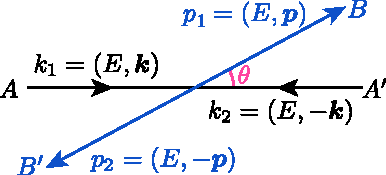
\includegraphics[width=\linewidth,page=1]{figs/collision.pdf}
\end{wrapfigure}

\noindent
For ``same mass'' collisions $(m_A,m_A)\to (m_1,m_1)$,
\begin{alignat*}{2}
t &= m_A^2+m_1^2 - s/2+2kp\cos\theta,\qquad
&k&={\sqrt{s/4-m_A^2}},\\
u &= m_A^2+m_1^2 - s/2-2kp\cos\theta,
&p&={\sqrt{s/4-m_1^2}}.
\end{alignat*}

\begin{wrapfigure}[2]{r}{12em}\vspace{-2em}
 \includegraphics[width=\linewidth,page=2]{figs/collision.pdf}
\end{wrapfigure}

\noindent
For ``initially massless'' collisions $(0,0)\to (m_1,m_2)$,
\begin{alignat*}{2}
 t &= (m_1^2+m_2^2-s)/2+p\sqrt{s}\cos\theta,\qquad
&p&=(\sqrt{s}/2)\Kallen[1/2](1,m_1^2/s,m_2^2/s),\\
 u &= (m_1^2+m_2^2-s)/2-p\sqrt{s}\cos\theta.
\end{alignat*}

\paragraph{Three-body final state} Mandelstam-like variables can be defined, for $P\to(p_1,p_2,p_3)$, as
\begin{equation*}
s_{ij}=(p_i+p_j)^2;\quad t_{0i}=(P-p_i)^2=s_{jk};\quad s_{12}+s_{23}+s_{31}=P^2+p_1^2+p_2^2+p_3^2.
\end{equation*}
For spherically-symmetric processes, the phase-space integral is reduced to, at the center-of-mass frame,
\begin{align}
\int\overline{\dd\Pi^3}_{\text{sph.\ sym.}}&(\sqrt{s}, \vc 0)
=\frac{1}{128\pi^3}\frac{1}{s}
\int_{(m_2+m_3)^2}^{(\sqrt{s}-m_1)^2}\dd s_{23}\int\dd s_{13};
\\ (s_{13})^{\text{max}}_{\text{min}} &=
\frac{(s+m_3^2-m_1^2-m_2^2)^2}{4s_{23}}
-\frac{1}{4s_{23}}
\left[\Kallen[1/2](s,m_1^2,s_{23})\mp\Kallen[1/2](s_{23},m_2^2,m_3^2)\right]^2
\notag\\&=(E_1^*+E_3^*)^2-\left(\sqrt{E_1^{*2}-m_1^2}\mp\sqrt{E_3^{*2}-m_3^2}\right)^2,
\quad
\end{align}
where 
$E_1^*=\frac{s-s_{23}-m_1^2}{2\sqrt{s_{23}}}$, and
$E_3^*=\frac{s_{23}-m_2^2+m_3^2}{2\sqrt{s_{23}}}$.


\newpage

\detailstyle
\subsection{Fundamentals}
Lorentz-invariant phase space:
\begin{equation*}
\int\dd\Pi
= \int\ddP{p}\frac{1}{2E_{\vc p}}
= \int\ddP{p}\frac{1}{2\sqrt{m^2+\|\vc p\|^2}}
= \int\frac{\dd p_0\dd^3\vc p}{(2\pi)^4}(2\pi)\diracdelta\left(p_0^2-\|\vc p\|^2-m^2\right)\Theta(p_0)
\end{equation*}
K\"all\'en function:
\begin{align*}
&\Kallen(x,y,z)
= x^2+y^2+z^2-2xy-2yz-2zx
= (x-y-z)^2-4yz;
\\
&
\Kallen(1;\alpha_1^2,\alpha_2^2)
= (1-(\alpha_1+\alpha_2)^2)(1-(\alpha_1-\alpha_2)^2)
= (1+\alpha_1+\alpha_2)(1-\alpha_1-\alpha_2)(1+\alpha_1-\alpha_2)(1-\alpha_1+\alpha_2).
\end{align*}
\begin{alignat*}{2}
&\Kallen[1/2]\left(s;m_1^2, m_2^2\right) = s\Kallen[1/2]\left(1;\frac{m_1^2}{s}, \frac{m_2^2}{s}\right);&
\qquad
&\Kallen[1/2]\left(1;\frac{m^2}{s},\frac{m^2}{s}\right)
= \sqrt{1-\frac{4 m^2}{s}},\\
&\Kallen[1/2]\left(1;\frac{m_1^2}{s},\frac{m_2^2}{s}\right)
= \sqrt{1-\frac{2 (m_1^2+m_2^2)}{s}+\frac{(m_1^2-m_2^2)^2}{s^2}},&
&\Kallen[1/2]\left(1;\frac{m_1^2}{s},0\right)
= \frac{s-m_1^2}{s}.
\end{alignat*}

\paragraph{Two-body phase space}
If $f(p_1^\mu,p_2^\mu)$ is Lorentz invariant, $f\equiv f(p_1^2,p_2^2,p_1^\mu p_{2\mu})\equiv f(p_1,p_2,\cos\theta_{12})$.
Meanwhile,
\begin{equation}
 \int\dd\Pi_1\dd\Pi_2
=
\int\ddP{p_1}\,\,\ddP{p_2}\frac{1}{2E_12E_2}
=
\int\frac{(4\pi)\dd p_1\,p_1^2}{(2\pi)^3}
\frac{(2\pi)\dd p_2\,p_2^2\,\dd\cos\theta_{12}}{(2\pi)^3}\frac{1}{2E_12E_2}
=
\int\frac{\dd E_+\dd E_- \dd s}{128\pi^4},
\end{equation}
with the replacement of the variables
\begin{align*}
& E_\pm = E_1\pm E_2,
\qquad
s=(p_1+p_2)^2=m_1^2 + m_2^2 + 2E_1E_2 - 2\|\vc p_1\|\|\vc p_2\|\cos\theta_{12};\\
&
\left|\frac{\dd(E_+,E_-,s)}{\dd(p_1, p_2, \cos\theta_{12})}\right|=\frac{4p_1^2p_2^2}{E_1E_2},
\qquad
\left|\frac{\dd(E_1,E_2,s)}{\dd(p_1, p_2, \cos\theta_{12})}\right|=\frac{2p_1^2p_2^2}{E_1E_2}.
\end{align*}
Therefore, 
\begin{equation}
 \int\dd\Pi_1\dd\Pi_2
=
\frac{1}{128\pi^4}
\int_{(m_1+m_2)^2}^\infty\dd s
\int_{\sqrt{s}}^\infty\dd E_+
\int\w{min}^{\mathrm{max}}\dd E_-,
\end{equation}
where the boundary of $E_-$ is given by
\begin{align*}
 &\cos\theta_{12}=\frac{E_+^2-E_-^2+2 \left(m_1^2+m_2^2-s\right)}{\sqrt{(E_++E_-)^2-4 m_1^2}\sqrt{(E_+-E_-)^2-4 m_2^2}} \in [-1,1]\\
 &\therefore\quad
\left|E_- - \frac{m_1^2-m_2^2}{s}E_+\right| 
\le
\sqrt{E_+^2-s}\cdot\Kallen[1/2]\left(1;\frac{m_1^2}{s},\frac{m_2^2}{s}\right)
=
2p\sqrt{\frac{E_+^2-s}{s}}.
\end{align*}

\paragraph{Two-body phase space with momentum conservation}
In a frame with total four-momentum being $(E_0,\vc P_0)$,
\begin{equation}
\overline{\dd\Pi^2}
=\frac{\dd^3\vc p_1}{16\pi^2}\frac{\delta(E_0-\sqrt{m_1^2+p_1^2}-\sqrt{m_2^2+\|\vc P_0-\vc p_1\|^2})}{E_1E_2}
=\frac{1}{8\pi}\frac{\dd E_1}{P_0}
~~\left(=\frac{1}{8\pi}\frac{p_1^2\dd\cos\theta_{1}}{E_0p_1-P_0E_1\cos\theta_1}\right),
\label{eq:twobodypsgeneral}
\end{equation}
where $\cos\theta_1$ and $p_1$ are related by
\begin{equation}
 2P_0 p_1\cos\theta_1 = 2E_0 \sqrt{p_1^2+m_1^2}-\mathcal M;
\qquad \mathcal M \coloneq  E_0^2 - P_0^2 +  m_1^2 - m_2^2.
\label{eq:twobodyanglemomentum}
\end{equation}
If $\vc P_0=\vc 0$, \cref{eq:twobodyanglemomentum} fixes $p_1$ and any $\theta_1$ is allowed, which is the CM result ($E_0=\sqrt s$).
Otherwise, \cref{eq:twobodyanglemomentum} associates $\theta_1$ with zero, one, or two values of $p_1$:
\begin{equation}
 \cos\theta_1 = \frac{2E_0E_1-\mathcal M}{2P_0p_1},\qquad
p_1=\frac{\mathcal MP_0\cos\theta_1
 \pm \mathcal R E_0
}{2(E_0^2-P_0^2\cos^2\theta_1)},\qquad
E_1=\frac{\mathcal ME_0
 \pm \mathcal RP_0\cos\theta_1
}{2(E_0^2-P_0^2\cos^2\theta_1)}
\end{equation}
with $\mathcal R = \sqrt{\mathcal M^2-4m_1^2(E_0^2-P_0^2\cos^2\theta_1)}$.

\subsection{Decay rate and Cross section}
As
$\braket{\text{out}|\text{in}}=(2\pi)^4\diracdelta[4](p\w i-p\w f)\ii\mathcal M$
(for $\text{in}\neq\text{out}$) and $\braket{\vc p|\vc p}=2E_{\vc p}(2\pi)^3\diracdelta[3](\vc 0)=2E_\vc {p}V$ for one-particle state,
\begin{equation}
 \frac{N\w{ev}}{\prod\w{in} N\w{particle}}
= \int\dd\Pi^{\mathrm{out}}\frac{\left|\braket{\text{out}|\text{in}}\right|^2}{\braket{\text{in}|\text{in}}}
= \int\dd\Pi^{\mathrm{out}}\frac{(2\pi)^8|\mathcal M|^2}{\prod\w{in}(2E)V}
\frac{VT}{(2\pi^4)}\diracdelta[4](p\w i-p\w f)
= VT\int\overline{\dd\Pi^{N\w f}}\frac{|\mathcal M|^2}{\prod\w{in}(2E)V}.
\end{equation}
Therefore, decay rate (at the rest frame) is given by
\begin{equation}
 \dd\Gamma
\coloneq  \frac{1}{T}\frac{\dd N\w{ev}}{N\w{particle}}
 = \frac{1}{T}VT\overline{\dd\Pi^{N\w f}}\frac{|\mathcal M|^2}{(2E)V}
 = \frac{1}{2M_0}\overline{\dd\Pi^{N\w f}}{|\mathcal M|^2}.
\end{equation}
We also define Lorentz-invariant cross section $\sigma$ by $N\w{ev}\eqcolon(n_A v_{\text{M\o l}}T\sigma)N_B=(n_A v_{\text{M\o l}}T\sigma)(n_B V)$ with
number density $n$, or
\begin{equation}
\dd\sigma\coloneq \frac{\dd N\w{ev}}{n_A v_{\text{M\o l}}TN_B}
=
\frac{V}{v_{\text{M\o l}}T}
VT\overline{\dd\Pi^{N\w f}}\frac{|\mathcal M|^2}{2E_A2E_BV^2}
=
\frac{1}{2E_A2E_B\,v_{\text{M\o l}}}
\overline{\dd\Pi^{N\w f}}|\mathcal M|^2.
\end{equation}
where the M\o ller parameter $v_{\text{M\o l}}$ is equal to $v^{\mathrm{NR}}\w{rel}=\|\vc v_A-\vc v_B\|$ if $\vc v_A\parallel\vc v_B$ (cf.~Ref.~\cite{Cannoni:2016hro}).
Generally,
\begin{equation}
  v_{\text{M\o l}}\coloneq 
 \frac{\sqrt{(p_A\cdot p_B)^2-m_A^2m_B^2}}{E_AE_B}
=\frac{\sqrt{\Kallen(s,m_A^2,m_B^2)}}{2E_AE_B}
=\frac{p_A\cdot p_B}{E_A E_B}v\w{rel}
=({1-\vc v_A\cdot\vc v_B})v\w{rel},
\end{equation}
where $v\w{rel}$ is the actual relative velocity
\begin{equation}
  v\w{rel}
=\sqrt{1-\frac{(1-v_A^2)(1-v_B^2)}{1-(\vc v_A\cdot\vc v_B)^2}}
=\frac{\sqrt{\|\vc v_A-\vc v_B\|^2-\|\vc v_A\times\vc v_B\|^2}}{1-\vc v_A\cdot\vc v_B}
=\frac{\Kallen[1/2](s,m_A^2,m_B^2)}{s-(m_A^2+m_B^2)}\neq v^{\mathrm{NR}}\w{rel}.
\end{equation}
(Note that $p_A\cdot p_B/E_AE_B=1$ if $\vc p_A=0$ or $\vc p_B=0$. Also, Each of $v\w{rel}$, $VT$, and $E_AE_Bv_{\text{M\o l}}$ is Lorentz invariant.)


\subsection{Three body phase space}
The phase-space reduction utilizes the identity~\cite{Hitoshi233B}
\begin{align}
 1
&= \int\frac{\dd^4 p_{ij}}{(2\pi)^4}(2\pi)^4\diracdelta[4](p_{ij}-p_i-p_j)\Theta(p_{ij}^0)
\\
&= \int\frac{\dd^4 p_{ij}}{(2\pi)^4}
\left[\int\frac{\dd s}{2\pi}(2\pi)\diracdelta(s-p_{ij}^2)\right]
(2\pi)^4\diracdelta[4](p_{ij}-p_i-p_j)\Theta(p_{ij}^0)
\\
&= \int\ddP{p_{ij}}
\frac{\dd s}{2\pi}\frac{1}{2p_{ij}^0}
(2\pi)^4\diracdelta[4](p_{ij}-p_i-p_j)\Big|_{p_{ij}^0=\sqrt{s+\|\vc p_{ij}\|^2}}.
\end{align}

For three-body phase space,
\begin{align}
\begin{split}
  \overline{\dd\Pi^3}
 &= \int\dd\Pi_1
 \frac{\dd^4 p_2\dd^4 p_3}{(2\pi)^8}
 (2\pi)\diracdelta(p_2^2-m_2^2)
 (2\pi)\diracdelta(p_3^2-m_3^2)
 \Theta(p_2^0)\Theta(p_3^0)
 (2\pi)^4\diracdelta[4]\left(P-p_1-p_2-p_3\right)
 \\&\qquad\times
\ddP{p_{23}}
\frac{\dd s_{23}}{2\pi}\frac{1}{2p_{23}^0}
(2\pi)^4\diracdelta[4](p_{23}-p_2-p_3)\Big|_{p_{23}^0=\sqrt{s_{23}+\|\vc p_{23}\|^2}}
\end{split}
\\
\begin{split}
 &= \int
\frac{\dd s_{23}}{2\pi}
\int
\dd\Pi_1
\ddP{p_{23}}
\frac{1}{2p_{23}^0}
 (2\pi)^4\diracdelta[4](P-p_1-p_{23})
\Big|_{p_{23}^0=\sqrt{s_{23}+\|\vc p_{23}\|^2}}
 \\&\qquad\times
 \frac{\dd^4 p_2\dd^4 p_3}{(2\pi)^8}
 (2\pi)\diracdelta(p_2^2-m_2^2)
 (2\pi)\diracdelta(p_3^2-m_3^2)
 \Theta(p_2^0)\Theta(p_3^0)
(2\pi)^4\diracdelta[4](p_{23}-p_2-p_3).
\end{split}
\\ &= \int
\frac{\dd s_{23}}{2\pi}
\int
\dd\Pi_1
\ddP{p_{23}}
\frac{1}{2p_{23}^0}
 (2\pi)^4\diracdelta[4](P-p_1-p_{23})
\Big|_{p_{23}^0=\sqrt{s_{23}+\|\vc p_{23}\|^2}}
\times \overline{\dd\Pi^2}(p^0_{23}, \vc p_{23})
\end{align}
and $\overline{\dd\Pi^2}(p^0_{23}, \vc p_{23})$ is given by \cref{eq:twobodypsgeneral}; explicitly,
\begin{align}
& \overline{\dd\Pi^2}(p^0_{23}, \vc p_{23}) = 
\frac{\dd\cos\theta_{2}}{8\pi}
\frac{p_{2}^2}{p^0_{23}p_2 - \|\vc p_{23}\|\sqrt{p_2^2+m_2^2}\cos\theta_2};
\\
&
p_2=\frac{(s_{23}+m_2^2-m_3^2)\|\vc p_{23}\|\cos\theta_2
 + p_{23}^0\sqrt{\Kallen(s_{23},m_2^2,m_3^2)-4m_2^2 \|\vc p_{23}\|^2 \sin^2\theta_2}
}{2(s_{23}+\|\vc p_{23}\|^2\sin^2\theta_2)},
\end{align}
where $\theta_2$ is the angle between $\vc p_{23}$ and $\vc p_2$ (in the lab frame).


If the matrix element to integrate is spherically symmetric, so as $\overline{\dd\Pi^2}(p^0_{23}, \vc p_{23})|\mathcal M|^2$, i.e., it is independent of the angle of $\vc p_{23}$. Then one can simply evaluate  $\int\dd^3\vc p_{23}$, which leads to, in the center-of-mass frame,
\begin{equation}
\overline{\dd\Pi^3}_{\text{sph.\ sym.}}(\sqrt{s}, \vc 0)
=
\frac{\dd s_{23}\dd\cos\theta_{2}}{64\pi^3}
\frac{p_1}{\sqrt s}
\frac{p_{2}^2}{p_2\sqrt{s_{23}+p_1^2} - p_1\sqrt{p_2^2+m_2^2}\cos\theta_2}\Big|_{
 p_1^2=\lambda(s,m_1^2,s_{23})/4s
}
= \frac{s}{128\pi^3}\dd x_1\dd x_2,
\end{equation}
where we defined $x_i\coloneq {2E_i}/{\sqrt s}$. Noting that $s_{23}=s+m_1^2-2E_1\sqrt{s}=s(1-x_1)+m_1^2$ etc., 
\begin{equation}
 \overline{\dd\Pi^3}_{\text{sph.\ sym.}}(\sqrt{s}, \vc 0)
=
\frac{1}{128\pi^3}\frac{1}{s}
\int_{(m_2+m_3)^2}^{(\sqrt{s}-m_1)^2}\dd s_{23}\int\dd s_{13};
\end{equation}
\begin{equation}
 (s_{13})^{\text{max}}_{\text{min}} =
\frac{(s+m_3^2-m_1^2-m_2^2)^2}{4s_{23}}
-\frac{1}{4s_{23}}
\left[\Kallen[1/2](s,m_1^2,s_{23})\mp\Kallen[1/2](s_{23},m_2^2,m_3^2)\right]^2.
\end{equation}
This is equal to the PDG-Eq.~(47.23)\cite{PDG2018}.


\subsection{Two-body decay of boosted particles}
A particle with $(P, \Theta, \Phi; M)$ decaying to two particles; at the CM frame the momenta of the decay products are characterized by $\vc q=(q,\theta,\phi)$ with $q=(M_0/2)\Kallen[1/2](1,m_1^2/M_0^2,m_2^2/M_0^2)$. Their lab-frame momenta are given by
\begin{align}
 P &=
\begin{pmatrix}
  E_0\\
 {P_0} \si\Theta \co\Phi \\
 {P_0} \si\Theta \si\Phi \\
 {P_0} \co\Theta \\
\end{pmatrix},&
 p_1&=
\begin{pmatrix}
  ({E_0 \mathcal{E}_1+P_0 q \co\theta})/{M_0} \\
 q \co\Theta \co\Phi \si\theta \co\phi - q \si\Phi \si\theta \si\phi + r_1 \si\Theta \co\Phi \\
 q \co\Theta \si\Phi \si\theta \co\phi + q \co\Phi \si\theta \si\phi   + r_1 \si\Theta \si\Phi \\
 -q \si\Theta \si\theta \co\phi + r_1 \co\Theta\\
\end{pmatrix},&
p_2&=
\begin{pmatrix}
  ({E_0 \mathcal{E}_2-P_0 q \co\theta})/{M_0} \\
 -q \co\Theta \co\Phi \si\theta \co\phi + q \si\Phi \si\theta \si\phi + r_2 \si\Theta \co\Phi \\
 -q \co\Theta \si\Phi \si\theta \co\phi - q \co\Phi \si\theta \si\phi + r_2 \si\Theta\si\Phi  \\
  q \si\Theta \si\theta \co\phi+r_2 \co\Theta \\
\end{pmatrix}
\end{align}
with $r_1=(P_0\mathcal{E}_1+E_0q\co\theta)/M_0$, $r_2=(P_0\mathcal{E}_2-E_0q\co\theta)$, and $\mathcal{E}_i=\sqrt{m_i^2+q^2}$.


\end{document}
